\scanpage{35}
\mspage{2}
\textcircled{4} \(\nu=2\). \deleted{There are \unsure{two cases}} \inserted{\unsure{In this case|In the}} \(K^g=\{P\}\), and \(K\setminus K^g\) \inserted{\(=I\)} is a union of two orbits. Thus, \(g\) is a ``universal'' automorphism \deleted{\unsure{of}} of \(\Sigma\setminus I\) (\(g\in V(\unsure{D_I|\mathbb D_I})\)) and \(P\) is \inserted{\unsure{one of|a|another}} \unsure{\deleted{a}|a} fixed poin\textsuperscript{t}. \deleted{\unsure{Of|This}} This time, the situation \unsure{has} ``moduli'', for example by choosing one of the two orbits,

\deleted{\unsure{one may assume} \unsure{that|for} the action of \(\unsure{g|\langle g\rangle}\) on it is that of \(\mu_2\) \inserted{\(=\{\pm1\}\)} on \(\mu_2\) \inserted{\(=\unsure{\{\pm1\}|(\pm1)}\)}, and \(P=0\), the other orbit is \deleted{\unsure{given by}} \unsure{a|a} \(\{t,-t\}\), with \(\lambda=t^2\ne1,\lambda\in k^\times\) ---
hence \deleted{\(\lambda=\)} \(J=(0,\pm1,\pm\unsure{\sqrt\lambda|t})\) \deleted{\(\unsure{\sqrt\lambda,\sqrt\lambda)|\sqrt\lambda,-\sqrt\lambda)}\)}, with \(\lambda\in\Sigma(k)\setminus\{0,1,\infty\}\),
\unsure{If one|by} \deleted{\unsure{changes}} changes the choice of the orbit, one finds
\[
(0,\pm1,\pm\sqrt{1/\lambda}).
\]
Let us take the parameter \(\rho=\lambda+\frac1\lambda\), \inserted{\(\ne2\)}, hence \(\lambda^2-\rho\lambda+1=0\);
\deleted{\(\lambda=\frac12(\rho\pm\sqrt{\rho^2-4})\)},
one finds \((0,\pm1,\pm\sqrt{\frac12(\rho\pm\sqrt{\rho^2\unsure{-4}})})\).
\unsure{Eliminate|As} \(0,\infty\), and \unsure{two|the} \unsure{discriminant} \(\lambda\longrightarrow1\), or --- \unsure{as} \deleted{\(\unsure{f^\circ|\rho}\)} \(\lambda\), and
\(g(z)=\frac{\lambda}{z}\), fixed poin\textsuperscript{ts}}

Case less interesting than the preceding ones, \unsure{from the|from} our point of view, for there are moduli. When the structure \((\Sigma,I)\) is a square structure, one recovers either case \(2^\circ\) (if \(g\) leaves the two diagonals stable), or the case \inserted{of the vertices} of an \deleted{\unsure{square|case|cube}} equilateral spherical square, and of the midpoint of one of the edges. \inserted{Is this case \(1^\circ\) ?} When it is a tetrahedral structure, \(P\) is one of the \inserted{\(6\)} vertices of the associated octahedron.

\figure{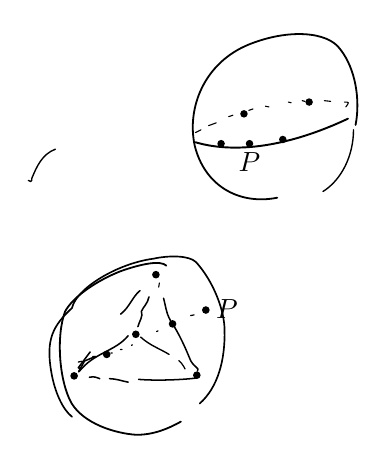
\begin{tikzpicture}[x=.0088cm,y=-.0088cm,line cap=round,line join=round]
% Upper sphere: the contour is open at lower right and has a short right-side gap.
\draw[line width=.65pt] (383,249)
 .. controls (327,260) and (278,231) .. (264,174)
 .. controls (252,119) and (278,54) .. (342,28)
 .. controls (399,5) and (456,9) .. (474,35)
 .. controls (496,63) and (503,108) .. (496,144);
\draw[line width=.5pt] (493,151)
 .. controls (493,188) and (476,223) .. (449,240);
\draw[line width=.7pt] (265,169)
 .. controls (323,186) and (400,175) .. (485,135);
% Rear equatorial arc, with the irregular short dashes visible on the sheet.
\draw[line width=.4pt] (265,155)--(273,151)
 (284,145)--(295,141) (313,132)--(319,130)
 (342,123)--(348,121) (366,117)--(371,118)
 (399,111)--(403,112) (419,109)--(423,110)
 (451,109)--(460,110) (480,111)..controls(487,111)..(482,118);
\foreach \x/\y in {302/171,343/171,391/165,335/128,429/111}
 {\fill (\x,\y) circle[radius=5.4];}
\node[below,inner sep=1pt] at (343,179) {$P$};
% Detached curved stroke at the left, without a supplied arrowhead.
\draw[line width=.5pt] (63,179)..controls(44,186)and(36,204)..(29,221)
 ..controls(30,227)and(25,226)..(24,224);
\begin{scope}[shift={(25,305)}]
% Lower sphere: the two left-hand contours and the open lower-right contour.
\draw[line width=.65pt] (198,42)
 ..controls(190,34)and(163,39)..(132,50)
 ..controls(99,63)and(64,86)..(52,108)
 ..controls(39,143)and(43,207)..(61,240)
 ..controls(79,270)and(124,284)..(155,286)
 ..controls(180,286)and(201,277)..(219,267);
\draw[line width=.6pt] (62,103)
 ..controls(34,129)and(24,149)..(32,195)
 ..controls(37,225)and(49,250)..(62,260);
\draw[line width=.6pt] (62,103)
 ..controls(68,75)and(127,39)..(179,32)
 ..controls(202,27)and(231,27)..(241,37)
 ..controls(267,66)and(282,108)..(282,135)
 ..controls(283,179)and(272,218)..(246,241);
% Broken outer triangular sides and rear branches, preserving their gaps.
\draw[line width=.55pt] (160,78)..controls(149,87)and(145,102)..(132,112);
\draw[line width=.55pt] (88.1778,166.4)--(71.1111,189.1556)--(74.6667,191.6444);
\draw[line width=.55pt] (71.4667,194.8444)--(80,179.5556)--(95.2889,173.1556);
\draw[line width=.55pt] (194,89)..controls(198,104)and(198,113)..(207,126)
 ..controls(216,140)and(224,157)..(231,174)
 ..controls(236,189)and(247,189)..(243,194);
\draw[line width=.55pt] (87,203)..controls(94,201)and(99,204)..(102,205)
 (116,205)..controls(126,205)and(136,209)..(143,210)
 (158,206)..controls(180,208)and(219,207)..(242,204);
\draw[line width=.55pt] (173,87)..controls(171,97)and(165,101)..(162,108)
 ..controls(165,115)and(159,122)..(157,130);
\draw[line width=.55pt] (143,143)..controls(124,166)and(94,167)..(72,195);
\draw[line width=.5pt] (161,145)..controls(174,157)and(189,162)..(202,170);
\draw[line width=.45pt] (216,179)..controls(220,182)and(223,187)..(225,191);
% Dotted oblique slant, including the short dash next to P.
\draw[line width=.45pt] (71,181)--(76,180) (92,173)--(97,173)
 (118,168)--(120,168) (132,163)--(134,163)
 (148,157)--(149,156) (184,137)--(186,136)
 (233,114)--(238,113);
\draw[line width=.4pt] (188,67)--(187,73);
\foreach \x/\y in {183/55,65/201,242/200,154/141,112/170,207/126,255/106}
 {\fill (\x,\y) circle[radius=5.5];}
\node[right,inner sep=2pt] at (261,105) {$P$};
\end{scope}
\end{tikzpicture}}

\uline{Case of the antiautomorphisms \inserted{\(\sigma\)} of} \(\Sigma\) leaving \(K\) \uline{stable}. \inserted{\unsure{(}Case \(k=\mathbb C\))} Since \unsure{it|\(\sigma\)} is of even order, one sees that it \deleted{\unsure{and|has}} \unsure{has|.} at least one fixed poin\textsuperscript{t} in \(K\), hence in \(\Sigma\), and being of finite order, one knows that it is of order \(2\), it corresponds to a real structure on \(\Sigma\), \deleted{\unsure{and}}
One distinguishes according to the cardinality of \(K^\sigma\), which is \(1,3\), or \(\unsure{6|5}\).
\margin{34}
